\clearpage

\lehead[]{\normalfont\sffamily\hspace*{-2.00cm}\textcolor{white}{\colorbox{lightblue}{\parbox[c][0.70cm][b]{1.60cm}{
\makebox[1.60cm][r]{\thechapter}\\ \makebox[1.60cm][r]{ÜBUNG}}}}\hspace{0.17cm}\textcolor{lightblue}{\chaptertitle}}
\rohead[]{\textcolor{lightblue}{\chaptertitle}\normalfont\sffamily\hspace*{0.17cm}\textcolor{white}{\colorbox{lightblue}{\parbox[c][0.70cm][b]{1.60cm}{\thechapter\\
ÜBUNG}}}\hspace{-2.00cm}}
%\chead[]{}
\rehead[]{\textcolor{lightblue}{AvHG, Inf, My}}
\lohead[]{\textcolor{lightblue}{AvHG, Inf, My}}

\section{Datenkapselung -- Übungen}

Die folgenden Übungsaufgaben sollen nach dem Prinzip der Datenkapselung programmiert werden.


\subsection{Aufgabe 1: Auf ein Haus zufahren}

\begin{compactenum}[a)]
\begin{minipage}{0.75\textwidth}
\item Schreibe eine Klasse, die ein einfaches Haus darstellt.

Vorgaben :

Das Haus soll durch folgende private Variablen beschrieben werden:

\begin{lstlisting}
private int x, y;    æ// x und y Position der linken unteren Ecke
æprivate int hoehe;   æ// Höhe des Hauses
\end{lstlisting}

Das Hinzufügen weiterer Hilfsvariablen ist erlaubt. Auch die Hilfsvariablen
müssen selbstverständlich versteckt werden.
\end{minipage}
\begin{minipage}{0.25\textwidth}
\begin{center}
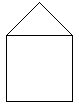
\includegraphics[width=0.5\textwidth]{./inf/SEKII/12_Java_Datenkapselung/haus.png}
\end{center}
\end{minipage}

\vspace{3mm}

Folgende Methoden sind notwendig:

\begin{compactenum}[1)]
\item Schreibe einen Konstruktor, durch den die Position des Hauses und die
anfängliche Höhe gesetzt werden können.
\item Schreibe eine Methode zum Zeichnen des Hauses mit den aktuellen
Einstellungen.
\item Die Höhe des Hauses soll nachträglich verändert werden können. Dabei soll
jedoch die linke untere Ecke des Hauses unverändert bleiben. Außerdem soll die
Breite des Hauses proportional mit verändert werden. Schreibe eine Methode zum
Auslesen der aktuellen Höhe und eine Methode zum Verändern der Höhe.
\end{compactenum}

\item Erzeuge in einem Anwendungsfenster ein Objekt der Klasse \myClass{Haus}.
Zeichne das Haus in der \lstinline|myPaint()|-Methode und erhöhe anschließend
die Höhe z.B.\ um 50 Pixel. Wenn man bei der laufenden Anwendung das
Anwendungsfenster kurz verdeckt und anschließend wieder sichtbar macht, ruft
das System die \lstinline|myPaint()|-Methode zum zweiten Mal auf und das Haus
muss nun größer erscheinen.

\item Füge in das Anwendungsfenster ein Objekt der Klasse \myClass{Timer} ein.
Verändere die \lstinline|myPaint()|-Methode des Anwendungsfenster so, dass das
Haus nach und nach immer größer wird, so als würde man in einem Auto auf das
Haus zufahren. Lese dazu bei jedem Aufruf der \lstinline|myPaint()|-Methode die
aktuelle Höhe des Hauses mit der entsprechenden \myClass{Haus}-Methode aus und
erhöhe den Wert um 1.
\end{compactenum}


\subsection{Aufgabe 2: Lampe}

\begin{minipage}{0.7\textwidth}
Programmiere eine Klasse \myClass{Lampe}, die anschließend in den beiden
nachfolgenden Aufgaben verwendet wird. Eine Lampe besitzt Attribute für
die x-Position, die y-Position und die Farbe. Die Breite der Lampe wird mit
einer Konstanten festgelegt. Außerdem besitzt die Lampe eine boolesche
Variable, die angibt ob die Lampe an oder aus ist. Alle Attribute sind
\lstinline|private|.

Im Konstruktor der Lampe kann man die Farbe und die Position der Lampe
festlegen. Es gibt Methoden zum Anschalten und Ausschalten der Lampe,
die den Wert der internen Variablen entsprechend verändern. Es gibt
außerdem eine Methode, mit der man abfragen kann, ob die Lampe an oder
aus ist. Die Methode \lstinline|zeichnen()| zeichnet die Lampe als ausgefüllten
Kreis. Wenn das Licht an ist, wird die Lampe in ihrer Farbe gezeichnet.
Andernfalls wird die Lampe mit grauer Farbe gezeichnet.

Erzeuge zum Test in einem Anwendungsfenster ein Objekt der Klasse
\myClass{Lampe} und schalte die Lampe in einer kleinen Animation immer
abwechselnd an und aus.
\end{minipage}
\begin{minipage}{0.3\textwidth}
\begin{center}
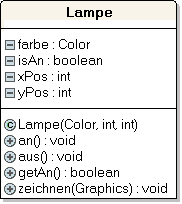
\includegraphics[width=0.9\textwidth]{./inf/SEKII/12_Java_Datenkapselung/lampeUML.png}
\end{center}
\end{minipage}


\subsection{Aufgabe 3: Ampel}

\begin{minipage}{0.9\textwidth}
Es ist eine Ampel zu programmieren, die in regelmäßigen Zeitabständen ihre
Farben ändert: rot, rot/gelb, grün, gelb, rot, usw.. Eine Ampel besitzt drei
verschiedene Objekte der Klasse \myClass{Lampe}: eine rote Lampe, eine gelbe
Lampe und eine grüne Lampe. Das Ein- und Ausschalten der Lampen wird von der
Ampel aus gesteuert. Die Ampel besitzt eine Methode \lstinline|umschalten()|,
die vom Anwendungsfenster im Sekunden-Takt aufgerufen wird. Sie schaltet dann
die Farben um. Abgesehen von der Taktgebung soll die Haupt-Anwendung nichts
über die Interna einer Ampel wissen müssen.
\end{minipage}
\begin{minipage}{0.1\textwidth}
\begin{center}

\includegraphics[width=0.5\textwidth]{./inf/SEKII/12_Java_Datenkapselung/ampel.png}
\end{center}
\end{minipage}

\vspace{1mm}

Erzeuge ein Anwendungsfenster, dass ein Objekt der Klasse \myClass{Ampel}
darstellt.

Zusatzaufgabe: Erzeuge mehrere Objekte der Klasse \myClass{Ampel} und
programmiere die Ampel so, dass die Ampeln mit unterschiedlichen
Anfangszuständen anfangen.


\subsection{Aufgabe 4: Lichterkette}

Programmiere eine Klasse \myClass{Lichterkette}. Eine Lichterkette besteht aus
einer Reihe verschiedenfarbiger Lampen-Objekte, die in regelmäßigen Abständen an und aus gehen.
Wichtig: Die Lampen sind in der Klasse \myClass{Lichterkette} „versteckt“, 
d.h.\ sie sind private. Die Lichterkette ist für die Haupt-Anwendung eine „Black
Box“, über deren Inneres sie nichts weiß.

Die Klasse \myClass{Lichterkette} besitzt einen Konstruktor, in dem die Position
der Lichterkette festgelegt werden kann. Außerdem gibt es (öffentliche)
Methoden zum Zeichnen der Lichterkette und zum An- und Ausschalten der Lichter.

Erzeuge im Anwendungsfenster mehrere Objekte der Klasse \myClass{Lichterkette}.


\subsection{Aufgabe 5: Digitaluhr}

Programmiere eine Digitaluhr mit vier Ziffern: zwei Ziffern zum Zählen der
Minuten und zwei Ziffern zum Zählen der Sekunden. Programmiere für die Ziffern
eine eigene Klasse und erzeuge in der Klasse Digitaluhr vier Objekte der Klasse
\myClass{Ziffer}.

\begin{minipage}{0.1\textwidth}
\begin{center}

\includegraphics[width=1.\textwidth]{./inf/SEKII/12_Java_Datenkapselung/digitaluhr.png}
\end{center}
\end{minipage}

Entwurf für die Digitaluhr

\begin{minipage}{1.0\textwidth}
\begin{center}
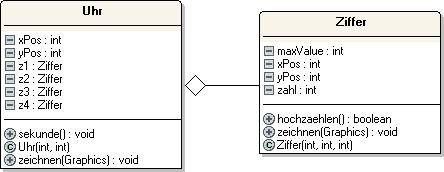
\includegraphics[width=0.7\textwidth]{./inf/SEKII/12_Java_Datenkapselung/digitaluhrUML.png}
\end{center}
\end{minipage}

\vspace{10mm}

Beschreibung der Klasse \myClass{Ziffer}:

\begin{compactenum}[a)]
\item Variablen

\begin{lstlisting}
private int xPos, yPos;     æ// linke untere Ecke in Pixel
æprivate int zahl;           æ// die aktuelle Ziffer
æprivate int maxValue;       æ// höchster Wert, den die Ziffer annehmen kann
                            // (je nach Stellung der Ziffer 5 oder 9)
\end{lstlisting}

\item Methoden

\begin{lstlisting}
public Ziffer(int x, int y, int maxValue) æ// Konstruktor
æpublic void zeichnen(Graphics g)          æ// zeichnet die Ziffer mit aktueller Zahl
æpublic boolean hochzaehlen()              æ/* Zählt die Ziffer um 1 hoch. Wenn die                                            
                                            höchste Zahl (maxValue) überschritten
                                            wird, wird die Ziffer auf 0 gesetzt.
                                            Der Rückgabewert gibt an, ob die Ziffer
                                            auf 0 gesetzt wurde  (true) oder nicht 
                                            (false). */
\end{lstlisting}
\end{compactenum}

Beschreibung der Klasse \myClass{Uhr}:

\begin{compactenum}[a)]
\item Variablen

\begin{lstlisting}
private int xPos, yPos;             æ// linke obere Ecke in Pixel
æprivate Ziffer z1, z2, z3, z4;      æ// die 4 Ziffern der Uhr
\end{lstlisting}

\item Methoden

\begin{lstlisting}
public Uhr(int x, int y)            æ// Konstruktor
æpublic void zeichnen(Graphics g)    æ// zeichnet die Uhr
æpublic void sekunde()               æ// erhöht die Zeit um eine Sekunde
\end{lstlisting}
\end{compactenum}



